\documentclass{ximera}

%\usepackage{todonotes}

\newcommand{\todo}{}

\usepackage{tkz-euclide}
\tikzset{>=stealth} %% cool arrow head
\tikzset{shorten <>/.style={ shorten >=#1, shorten <=#1 } } %% allows shorter vectors

\usepackage{tkz-tab}  %% sign charts
\usetikzlibrary{decorations.pathreplacing} 

\usetikzlibrary{backgrounds} %% for boxes around graphs
\usetikzlibrary{shapes,positioning}  %% Clouds and stars
\usetikzlibrary{matrix} %% for matrix
\usepgfplotslibrary{polar} %% for polar plots
\usetkzobj{all}
\usepackage[makeroom]{cancel} %% for strike outs
%\usepackage{mathtools} %% for pretty underbrace % Breaks Ximera
\usepackage{multicol}

\usepackage{polynom}



\usepackage[many]{tcolorbox}  %% for titled boxes
\newtcolorbox{xbox}[1]{%
    tikznode boxed title,
    enhanced,
    arc=0mm,
    interior style={white},
    attach boxed title to top center= {yshift=-\tcboxedtitleheight/2},
    fonttitle=\bfseries,
    colbacktitle=white,coltitle=black,
    boxed title style={size=normal,colframe=white,boxrule=0pt},
    title={#1}}


\usepackage{array}
\setlength{\extrarowheight}{+.1cm}   
\newdimen\digitwidth
\settowidth\digitwidth{9}
\def\divrule#1#2{
\noalign{\moveright#1\digitwidth
\vbox{\hrule width#2\digitwidth}}}





\newcommand{\RR}{\mathbb R}
\newcommand{\R}{\mathbb R}
\newcommand{\N}{\mathbb N}
\newcommand{\Z}{\mathbb Z}

%\renewcommand{\d}{\,d\!}
\renewcommand{\d}{\mathop{}\!d}
\newcommand{\dd}[2][]{\frac{\d #1}{\d #2}}
\newcommand{\pp}[2][]{\frac{\partial #1}{\partial #2}}
\renewcommand{\l}{\ell}
\newcommand{\ddx}{\frac{d}{\d x}}
\newcommand{\ddt}{\frac{d}{\d t}}

\newcommand{\zeroOverZero}{\ensuremath{\boldsymbol{\tfrac{0}{0}}}}
\newcommand{\inftyOverInfty}{\ensuremath{\boldsymbol{\tfrac{\infty}{\infty}}}}
\newcommand{\zeroOverInfty}{\ensuremath{\boldsymbol{\tfrac{0}{\infty}}}}
\newcommand{\zeroTimesInfty}{\ensuremath{\small\boldsymbol{0\cdot \infty}}}
\newcommand{\inftyMinusInfty}{\ensuremath{\small\boldsymbol{\infty - \infty}}}
\newcommand{\oneToInfty}{\ensuremath{\boldsymbol{1^\infty}}}
\newcommand{\zeroToZero}{\ensuremath{\boldsymbol{0^0}}}
\newcommand{\inftyToZero}{\ensuremath{\boldsymbol{\infty^0}}}



\newcommand{\numOverZero}{\ensuremath{\boldsymbol{\tfrac{\#}{0}}}}
\newcommand{\dfn}{\textbf}
%\newcommand{\unit}{\,\mathrm}
\newcommand{\unit}{\mathop{}\!\mathrm}
\newcommand{\eval}[1]{\bigg[ #1 \bigg]}
\newcommand{\seq}[1]{\left( #1 \right)}
\renewcommand{\epsilon}{\varepsilon}
\renewcommand{\iff}{\Leftrightarrow}

\DeclareMathOperator{\arccot}{arccot}
\DeclareMathOperator{\arcsec}{arcsec}
\DeclareMathOperator{\arccsc}{arccsc}
\DeclareMathOperator{\si}{Si}
\DeclareMathOperator{\proj}{proj}
\DeclareMathOperator{\scal}{scal}


\newcommand{\tightoverset}[2]{% for arrow vec
  \mathop{#2}\limits^{\vbox to -.5ex{\kern-0.75ex\hbox{$#1$}\vss}}}
\newcommand{\arrowvec}[1]{\tightoverset{\scriptstyle\rightharpoonup}{#1}}
\renewcommand{\vec}{\mathbf}
\newcommand{\veci}{\vec{i}}
\newcommand{\vecj}{\vec{j}}
\newcommand{\veck}{\vec{k}}
\newcommand{\vecl}{\boldsymbol{\l}}

\newcommand{\dotp}{\bullet}
\newcommand{\cross}{\boldsymbol\times}
\newcommand{\grad}{\boldsymbol\nabla}
\newcommand{\divergence}{\grad\dotp}
\newcommand{\curl}{\grad\cross}
%\DeclareMathOperator{\divergence}{divergence}
%\DeclareMathOperator{\curl}[1]{\grad\cross #1}


\colorlet{textColor}{black} 
\colorlet{background}{white}
\colorlet{penColor}{blue!50!black} % Color of a curve in a plot
\colorlet{penColor2}{red!50!black}% Color of a curve in a plot
\colorlet{penColor3}{red!50!blue} % Color of a curve in a plot
\colorlet{penColor4}{green!50!black} % Color of a curve in a plot
\colorlet{penColor5}{orange!80!black} % Color of a curve in a plot
\colorlet{fill1}{penColor!20} % Color of fill in a plot
\colorlet{fill2}{penColor2!20} % Color of fill in a plot
\colorlet{fillp}{fill1} % Color of positive area
\colorlet{filln}{penColor2!20} % Color of negative area
\colorlet{fill3}{penColor3!20} % Fill
\colorlet{fill4}{penColor4!20} % Fill
\colorlet{fill5}{penColor5!20} % Fill
\colorlet{gridColor}{gray!50} % Color of grid in a plot

\newcommand{\surfaceColor}{violet}
\newcommand{\surfaceColorTwo}{redyellow}
\newcommand{\sliceColor}{greenyellow}




\pgfmathdeclarefunction{gauss}{2}{% gives gaussian
  \pgfmathparse{1/(#2*sqrt(2*pi))*exp(-((x-#1)^2)/(2*#2^2))}%
}


%%%%%%%%%%%%%
%% Vectors
%%%%%%%%%%%%%

%% Simple horiz vectors
\renewcommand{\vector}[1]{\left\langle #1\right\rangle}


%% %% Complex Horiz Vectors with angle brackets
%% \makeatletter
%% \renewcommand{\vector}[2][ , ]{\left\langle%
%%   \def\nextitem{\def\nextitem{#1}}%
%%   \@for \el:=#2\do{\nextitem\el}\right\rangle%
%% }
%% \makeatother

%% %% Vertical Vectors
%% \def\vector#1{\begin{bmatrix}\vecListA#1,,\end{bmatrix}}
%% \def\vecListA#1,{\if,#1,\else #1\cr \expandafter \vecListA \fi}

%%%%%%%%%%%%%
%% End of vectors
%%%%%%%%%%%%%

%\newcommand{\fullwidth}{}
%\newcommand{\normalwidth}{}



%% makes a snazzy t-chart for evaluating functions
%\newenvironment{tchart}{\rowcolors{2}{}{background!90!textColor}\array}{\endarray}

%%This is to help with formatting on future title pages.
\newenvironment{sectionOutcomes}{}{} 



%% Flowchart stuff
%\tikzstyle{startstop} = [rectangle, rounded corners, minimum width=3cm, minimum height=1cm,text centered, draw=black]
%\tikzstyle{question} = [rectangle, minimum width=3cm, minimum height=1cm, text centered, draw=black]
%\tikzstyle{decision} = [trapezium, trapezium left angle=70, trapezium right angle=110, minimum width=3cm, minimum height=1cm, text centered, draw=black]
%\tikzstyle{question} = [rectangle, rounded corners, minimum width=3cm, minimum height=1cm,text centered, draw=black]
%\tikzstyle{process} = [rectangle, minimum width=3cm, minimum height=1cm, text centered, draw=black]
%\tikzstyle{decision} = [trapezium, trapezium left angle=70, trapezium right angle=110, minimum width=3cm, minimum height=1cm, text centered, draw=black]


\outcome{Interpert the product of rate and time as area.}
\outcome{Approximate position from velocity.}
\outcome{Recognize Riemann sums.}
\author{Nela Lakos}


\title[Dig-In:]{Relating velocity, displacement, antiderivatives and areas}


\begin{document}
\begin{abstract}
We give an alternative interpretation of the definite integral and
make a connection between areas and antiderivatives.
\end{abstract}
\maketitle

We have a geometric interpretation of the derivative as the slope of a
tangent line at a point.  We have not yet found a geometric
interpretation of antiderivatives.


\section{More than one perspective}

We'll start with a question:

\begin{question}
   Suppose you are in slow traffic moving at $4$ \textrm{mph} from
   $2$pm to $5$pm.  How far have you traveled?
   \begin{prompt}
     \[
     \text{displacement}= \answer{12}\ \text{miles}.
     \]
   \end{prompt}
   \begin{feedback}
     Since the (constant) velocity over a time interval is given by
     \[
     \text{velocity}=\frac{\text{displacement}}{\text{elapsed time}},
     \]
     it follows that the displacement of the object over an interval
     of time is given by
     \[
     \text{displacement}=\text{velocity}\cdot
     (\text{elapsed time}),
     \]  
     The graph of the (constant) velocity function $v$ on the interval
     $[2,5]$ is given in the figure.
      \begin{image}
        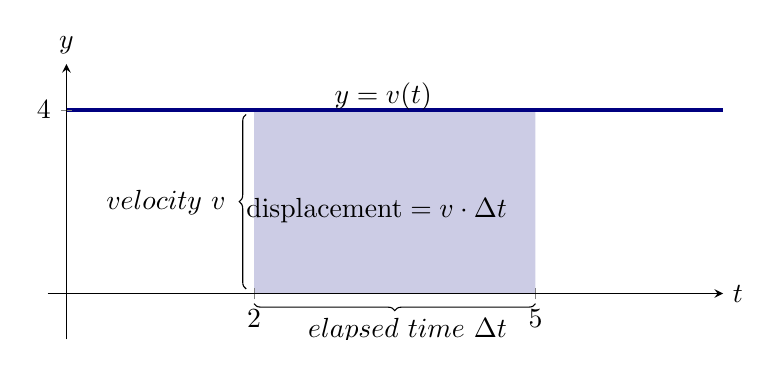
\begin{tikzpicture}[
            declare function = {f(\x) = 4;} ]
          \begin{axis}[
              domain=-.2:7, xmin =-.2,xmax=7,ymax=5,ymin=-1,
              width=4in, height=2in, xtick={2,5}, ytick={4},
              xticklabels={$2$,$5$}, yticklabels={$4$}, axis
              lines=center, xlabel=$t$, ylabel=$y$, every axis y
              label/.style={at=(current axis.above
                origin),anchor=south}, every axis x
              label/.style={at=(current axis.right of
                origin),anchor=west}, axis on top, ] \addplot
            [draw=none,fill=fillp,domain=2:5, smooth] {f(x)}
            \closedcycle; \addplot [ultra thick,penColor, smooth,
              domain=0:7] {f(x)}; \node[anchor=east] at (axis
            cs:4,4.3) {$y=v(t)$}; \node[anchor=east] at (axis
            cs:1.8,1.98) {$velocity$ $v$}; \node[anchor=east] at (axis
            cs:4.8,-0.8) {$elapsed$ $time$ $\Delta t$ };
            \node[anchor=east] at (axis cs:4.8,1.8)
                 {$\text{displacement}=v\cdot \Delta t$ };
                 \addplot[decoration={brace,raise=.1cm},decorate,thin]
                 plot coordinates {(2,.1) (2,{f(2)-.1})};
                 \addplot[decoration={brace,mirror,raise=.1cm},decorate,thin]
                 plot coordinates {(2,-0.05) (5,-0.05)};
        \end{axis}
\end{tikzpicture}
\end{image}

      So, the displacement of an object is given by the product of the  velocity and elapsed time, and is represented by the area of the shaded rectangle in the figure. 
      \end{feedback}
\end{question}
Since the displacement of an object moving at constant velocity
over a time interval can be represented by the area of a
rectangle, we can approximate displacement of an object moving
at nonconstant velocity using Riemann sums.  We explain this
process in detail in our next example.


%    
%    The fact that these two answers are the same is the germ of one of the
%    most ``fundamental'' ideas in all of calculus. However, before we can
%    step ahead, we might first look back to our even younger days of being mathematicians.
%    
%    Recall that there are (at least!) two basic models of multiplication:
%    A ``rate times time'' perspective and an ``area'' perspective.  For
%    instance, we could interpret
%    \[
%    4\times 3
%    \]
%    as an answer to the question:
%    \begin{quote}
%    If I am going $4 \textrm{mph}$ for $3$ hours, how far have I
%    traveled?
%    \end{quote}
%    or as the answer to the question
%    \begin{quote}
%    What is the area of a rectangle with height $4$ and width $3$?
%    \end{quote}
%    In what follows below, we will leverage these two different notions to
%    gain insight into our study of functions.
%    

%

\begin{example}
  Assume an object is moving along a straight line with the velocity
  $v(t)=\frac{t^2}{4}+1$, for $0\le t\le4$, where $t$ is measured in
  seconds, and $v$ in $\frac{\unit{ft}}{\unit{s}}$.
  
  Find the displacement of the object over the time interval $[0,4]$. 
  \begin{explanation}
   Since we know how to compute the displacement when the velocity is
   constant, we will start by asuming that the velocity is constant
   and equal to $v(0)$, the initial velocity, for the entire
   four-second time interval, $\Delta t=4$.
   
   This scenario will give us a very rough approximation of the
   displacement, but it is a good starting point.
  \[
   \text{displacement}\approx v(0)\cdot\Delta t=1\cdot(4-0)=4 \unit{ft}/\unit{s}
  \]
This scenario is illustrated in the figure below.
 \begin{image}
  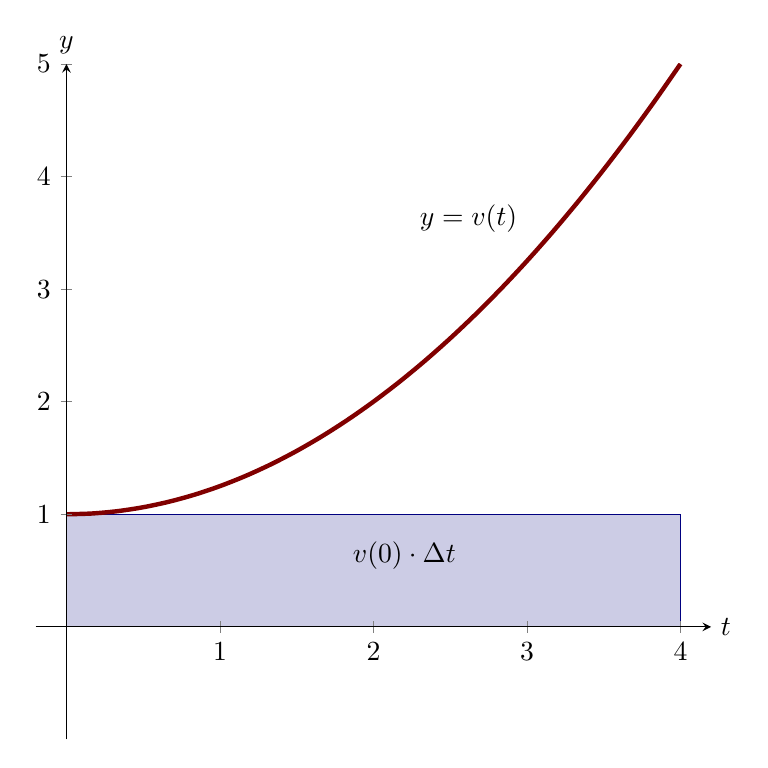
\begin{tikzpicture}[
      declare function = {f(\x) =(1/4)*(x^2) +1;} ]
	\begin{axis}[
            domain=-.2:4.2, xmin =-.2,xmax=4.2,ymax=5,ymin=-1,
            width=4in,
            height=4in,
            xtick={1,2,3,4}, 
	   ytick={1,2,3,4,5},
            xticklabels={1,2,3,4},
            yticklabels={1,2,3,4,5},
            axis lines=center, xlabel=$t$, ylabel=$y$,
            every axis y label/.style={at=(current axis.above origin),anchor=south},
            every axis x label/.style={at=(current axis.right of origin),anchor=west},
            axis on top,
          ]
          \addplot [draw=penColor,fill=fillp,domain=0:4, smooth] {1} \closedcycle;
          \addplot [ultra thick,penColor2, smooth, domain=0:4] {f(x)};
          

            \node[anchor=east] at (axis cs:3,3.63) {$y=v(t)$};
             \node[anchor=east] at (axis cs:2.6,0.63) {$v(0)\cdot\Delta t$ };
             % \node[anchor=east] at (axis cs:4.8,-0.8) {$elapsed$  $time$ $\Delta t$ };
              % \node[anchor=east] at (axis cs:4.8,1.8) {$displacement=v\cdot \Delta t$ };
           % \addplot[decoration={brace,raise=.1cm},decorate,thin] plot coordinates
                       {(-02,.1) (-0.2,{f(0)-.1})};
              % \addplot[decoration={brace,mirror,raise=.1cm},decorate,thin] plot coordinates
                       {(0,-0.05) (4,-0.05)};
        \end{axis}
\end{tikzpicture}
\end{image}
%At $t=2$, $s'(2) = v(2) = \answer[given]{6}$, so we attach a
%segment of slope $\answer[given]{6}$ over the next interval of
%length $2$:
%\begin{image}
%\begin{tikzpicture}[
%  declare function = {f(\x) = 6+ \x/2 - pow(\x,2)/4;} ]
%	\begin{axis}[
%        domain=0:10, xmin =0,xmax=10.2,ymax=45,ymin=-1,
%        width=6in,
%        height=3in,
%        xtick={0,2,4,6,8,10}, 
%        %xticklabels={$1$,$1.5$,$2$, $2.5$, $3$},
%        %% ytick style={draw=none},
%        %% yticklabels={},
%        axis lines=center, xlabel=$t$, ylabel=$y$,
%        every axis y label/.style={at=(current axis.above origin),anchor=south},
%        every axis x label/.style={at=(current axis.right of origin),anchor=west},
%      ]
%      \addplot [draw=penColor,ultra thick] plot coordinates {(0,0) (2,{f(0)*2})};
%      \addplot [draw=penColor2,ultra thick] plot coordinates {(2,{f(0)*2}) (4, {f(0)*2+f(2)*2})};
%
%      \addplot [draw=black,dashed,->,>=stealth'] plot coordinates {(2.1,12) (3.9, 12)};
%                
%      \addplot [draw=black,dashed,->,>=stealth'] plot coordinates {(4,13) (4, 23)};
%      
%      \node[anchor=west] at (axis cs:4,18) {\small${\color{penColor2}v(2)\cdot 2}$};
%                
%    \end{axis}
%\end{tikzpicture}
%\end{image}
%At $t=4$, $s'(4) = v(4) = \answer[given]{4}$, so we attach a
%segment of slope $\answer[given]{4}$ over the next interval of length $2$:
%\begin{image}
%\begin{tikzpicture}[
%  declare function = {f(\x) = 6+\x/2 - pow(\x,2)/4;} ]
%	\begin{axis}[
%        domain=0:10, xmin =0,xmax=10.2,ymax=45,ymin=-1,
%        width=6in,
%        height=3in,
%        xtick={0,2,4,6,8,10}, 
%        %xticklabels={$1$,$1.5$,$2$, $2.5$, $3$},
%        %% ytick style={draw=none},
%        %% yticklabels={},
%        axis lines=center, xlabel=$t$, ylabel=$y$,
%        every axis y label/.style={at=(current axis.above origin),anchor=south},
%        every axis x label/.style={at=(current axis.right of origin),anchor=west},
%      ]
%      \addplot [draw=penColor,ultra thick] plot coordinates {(0,0) (2,{f(0)*2})};
%      \addplot [draw=penColor2,ultra thick] plot coordinates {(2,{2*f(0)}) (4, {f(0)*2+f(2)*2})};
%      \addplot [draw=penColor3,ultra thick] plot coordinates {(4, {f(0)*2+f(2)*2}) (6, {f(0)*2+f(2)*2+f(4)*2})};
%
%
%      \addplot [draw=black,dashed,->,>=stealth'] plot coordinates {(4.1,24) (5.9, 24)};
%
%      
%
%      \addplot [draw=black,dashed,->,>=stealth'] plot coordinates {(6,25) (6, 31)};
%
%      
%
%      \node[anchor=west] at (axis cs:6,27) {\small${\color{penColor3}v(4) \cdot 2}$};
%      
%    \end{axis}
%\end{tikzpicture}
%\end{image}
%At $t=6$, $s'(6) = v(6) = \answer[given]{0}$, so we attach a segment of slope $\answer[given]{0}$ over the next interval of length $2$:
%\begin{image}
%\begin{tikzpicture}[
%  declare function = {f(\x) = 6+\x/2 - pow(\x,2)/4;} ]
%	\begin{axis}[
%        domain=0:10, xmin =0,xmax=10.2,ymax=45,ymin=-1,
%        width=6in,
%        height=3in,
%        xtick={0,2,4,6,8,10}, 
%        %xticklabels={$1$,$1.5$,$2$, $2.5$, $3$},
%        %% ytick style={draw=none},
%        %% yticklabels={},
%        axis lines=center, xlabel=$t$, ylabel=$y$,
%        every axis y label/.style={at=(current axis.above origin),anchor=south},
%        every axis x label/.style={at=(current axis.right of origin),anchor=west},
%      ]
%      \addplot [draw=penColor,ultra thick] plot coordinates {(0,0) (2,{f(0)*2})};
%      \addplot [draw=penColor2,ultra thick] plot coordinates {(2,{2*f(0)}) (4, {2*f(0)+f(2)*2})};
%      \addplot [draw=penColor3,ultra thick] plot coordinates {(4, {f(0)*2+f(2)*2}) (6, {f(0)*2+f(2)*2+f(4)*2})};
%      \addplot [draw=penColor4,ultra thick] plot coordinates {(6, {f(0)*2+f(2)*2+f(4)*2}) (8, {f(0)*2+f(2)*2+f(4)*2 + f(6)*2})};
%
%      \addplot [draw=black,dashed,->,>=stealth'] plot coordinates {(6.1,32) (7.9, 32)};
%                          
%      \node[anchor=east] at (axis cs:8,30) {\small${\color{penColor4}v(6)\cdot 2}$};
%      
%    \end{axis}
%\end{tikzpicture}
%\end{image}
%At $t=8$, $s'(8) = v(8) = \answer[given]{-6}$, so we attach a segment of slope $\answer[given]{-6}$ over the next interval of length $2$:
%\begin{image}
%\begin{tikzpicture}[
%  declare function = {f(\x) = 6+ \x/2 - pow(\x,2)/4;} ]
%	\begin{axis}[
%        domain=0:10, xmin =0,xmax=10.2,ymax=45,ymin=-1,
%        width=6in,
%        height=3in,
%        xtick={0,2,4,6,8,10}, 
%        %xticklabels={$1$,$1.5$,$2$, $2.5$, $3$},
%        %% ytick style={draw=none},
%        %% yticklabels={},
%        axis lines=center, xlabel=$t$, ylabel=$y$,
%        every axis y label/.style={at=(current axis.above origin),anchor=south},
%        every axis x label/.style={at=(current axis.right of origin),anchor=west},            
%      ]
%      \addplot [draw=penColor,ultra thick] plot coordinates {(0,0) (2,{f(0)*2})};
%      \addplot [draw=penColor2,ultra thick] plot coordinates {(2,{2*f(0)}) (4, {2*f(0)+f(2)*2})};
%      \addplot [draw=penColor3,ultra thick] plot coordinates {(4, {f(0)*2+f(2)*2}) (6, {f(0)*2+f(2)*2+f(4)*2})};
%      \addplot [draw=penColor4,ultra thick] plot coordinates {(6, {f(0)*2+f(2)*2+f(4)*2}) (8, {f(0)*2+f(2)*2+f(4)*2 + f(6)*2})};
%      \addplot [draw=penColor5,ultra thick] plot coordinates {(8, {f(0)*2+f(2)*2+f(4)*2 + f(6)*2}) (10,{f(0)*2+f(2)*2+f(4)*2 + f(6)*2 +f(8)*2} )};
%
%      \addplot [draw=black,dashed,->,>=stealth'] plot coordinates {(8.1,32) (9.9, 32)};
%
%      \addplot [draw=black,dashed,->, >=stealth'] plot coordinates {(10,31) (10, 21)};
%
%      \node[anchor=east] at (axis cs:10,28) {\small${\color{penColor5}v(8)\cdot 2}$};  
%      
%    \end{axis}
%\end{tikzpicture}
%\end{image}
%This gives us a plot of the approximate position of our object.
Now it should be clear how to proceed. We will keep approximating the velocity with a constant over smaller and smaller intervals of time.


In our next step we will assume that the velocity is constant during two-second time intervals $[0,2]$ and $[2,4]$. For each of these two intervals, we assume that the velocity is equal to the velocity at the beginning of the time interval.

In this case,  the object would move by $v(0)\cdot2 \unit{ft}$ during the time interval $[0,2]$, and during the next two seconds, the object would move by $v(2)\cdot2 \unit{ft}$.
 
  
If we let $\Delta t$ denote the length of the time interval, we can approximate the displacement  and write

  \[
   \text{displacement}\approx v(0)\cdot\Delta t+v(2)\cdot\Delta t=1\cdot2+2\cdot2=\answer[given]{6} \unit{ft}/\unit{s}
  \]
Using sigma notation, we write
\[
   \text{displacement}\approx \sum_{k=1}^2v((k-1)\cdot\Delta t)\Delta t
  \]
Since we evaluate the velocity at the sample points $t_{k}^*=(k-1)\cdot\Delta t$, $k=1,2$, we can also  write

\[
   \text{displacement}\approx \sum_{k=1}^2v(t_{k}^*)\Delta t.
  \]
  This is a left Riemann sum for the function $v$ on the interval $[0,4]$, when $n=2$.
This scenario is illustrated in the figure below.
\begin{image}
  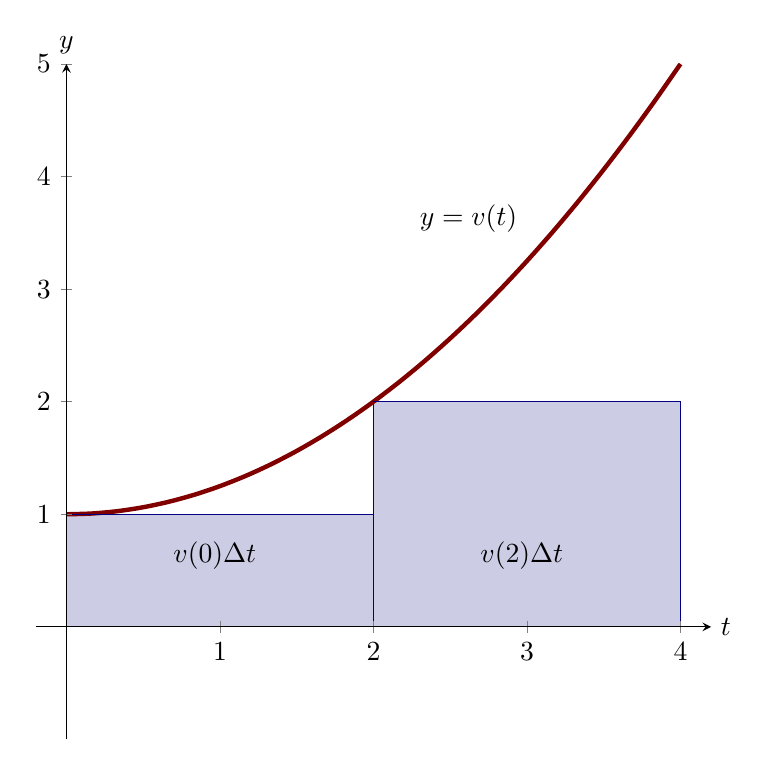
\begin{tikzpicture}[
      declare function = {f(\x) =(1/4)*(x^2) +1;} ]
	\begin{axis}[
            domain=-.2:4.2, xmin =-.2,xmax=4.2,ymax=5,ymin=-1,
            width=4in,
            height=4in,
            xtick={1,2,3,4}, 
	    ytick={1,2,3,4,5},
            xticklabels={1,2,3,4},
            yticklabels={1,2,3,4,5},
            axis lines=center, xlabel=$t$, ylabel=$y$,
            every axis y label/.style={at=(current axis.above origin),anchor=south},
            every axis x label/.style={at=(current axis.right of origin),anchor=west},
            axis on top,
          ]
          \addplot [draw=penColor,fill=fillp,domain=0:2, smooth] {1} \closedcycle;
          \addplot [draw=penColor,fill=fillp,domain=2:4, smooth] {2} \closedcycle;
          \addplot [ultra thick,penColor2, smooth, domain=0:4] {f(x)};
          \addplot [penColor, smooth, domain=0:2] {1};
          \addplot [penColor, smooth, domain=2:4] {2};
          \node[anchor=east] at (axis cs:1.3,0.63) {$v(0)\Delta t$};
          \node[anchor=east] at (axis cs:3.3,0.63) {$v(2)\Delta t$};
          \node[anchor=east] at (axis cs:3,3.63) {$y=v(t)$};
          %\node[anchor=east] at (axis cs:1.8,1.98) {$velocity$ $v$};
          % \node[anchor=east] at (axis cs:4.8,-0.8) {$elapsed$  $time$ $\Delta t$ };
          % \node[anchor=east] at (axis cs:4.8,1.8) {$displacement=v\cdot \Delta t$ };
          % \addplot[decoration={brace,raise=.1cm},decorate,thin] plot coordinates
               {(-02,.1) (-0.2,{f(0)-.1})};
               % \addplot[decoration={brace,mirror,raise=.1cm},decorate,thin] plot coordinates
               {(0,-0.05) (4,-0.05)};
        \end{axis}
\end{tikzpicture}
\end{image}
Next, we approximate the displacement of the object assuming that the velocity is constant during one-second time intervals, and that velocity is equal to the velocity at the beginning of each time interval.


Under this assumption, during the first second, the object would move
by $v(0)\cdot1 \unit{ft}$; during the second time interval of one
second, the object would move by $v(1)\cdot1 \unit{ft}$, during the
third second, the object would move by $v(2)\cdot1 \unit{ft}$, and
during the last second, it would move by $v(3)\cdot1 \unit{ft}$.
 
During the entire time interval, the object would move by
\begin{align*}
  \text{displacement} &\approx v(0)\cdot\Delta t+v(1)\cdot\Delta t+v(2)\cdot\Delta t+v(3)\cdot\Delta t\\
  &=\frac{\answer[given]{15}}{4} \unit{ft}/\unit{s}
\end{align*}
Using sigma notation and the fact that $\Delta t=\frac{4-0}{4}=1$, we can write
\[
   \text{displacement}\approx \sum_{k=1}^4v((k-1)\cdot\Delta t)\Delta t
  \]
  Again, we denote the  sample points by $t_{k}^*=(k-1)\cdot\Delta t$, $k=1,2,3,4$, and write
  \[
   \text{displacement}\approx \sum_{k=1}^4v(t_{k}^*)\Delta t
  \]
  This is a left Riemann sum for the function $v$ on the interval $[0,4]$, when $n=4$.
This scenario is illustrated in the figure below.
\begin{image}
  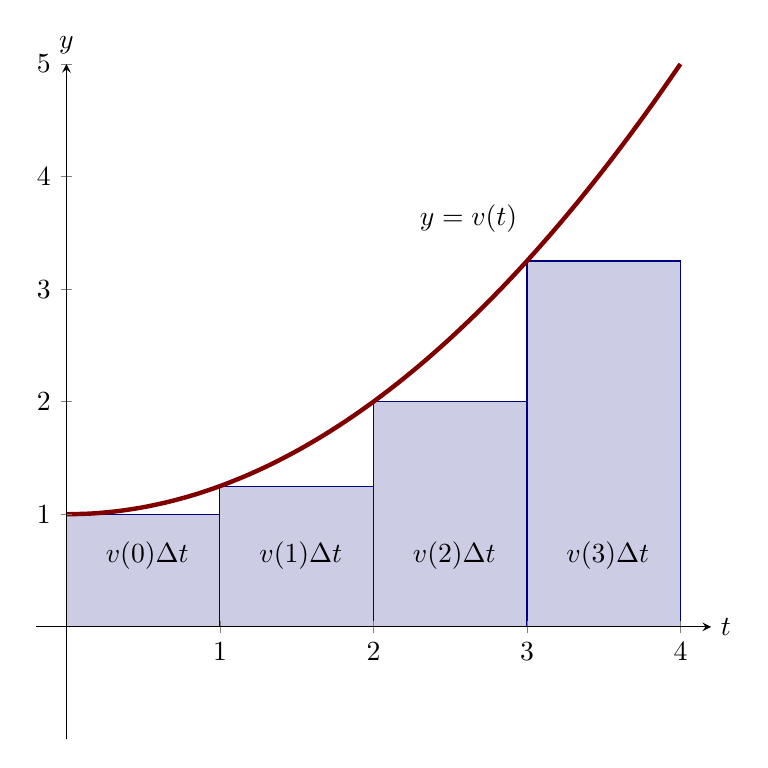
\begin{tikzpicture}[
      declare function = {f(\x) =(1/4)*(x^2) +1;} ]
	\begin{axis}[
            domain=-.2:4.2, xmin =-.2,xmax=4.2,ymax=5,ymin=-1,
            width=4in,
            height=4in,
            xtick={1,2,3,4}, 
	   ytick={1,2,3,4,5},
            xticklabels={1,2,3,4},
            yticklabels={1,2,3,4,5},
            axis lines=center, xlabel=$t$, ylabel=$y$,
            every axis y label/.style={at=(current axis.above origin),anchor=south},
            every axis x label/.style={at=(current axis.right of origin),anchor=west},
            axis on top,
          ]
          \addplot [draw=penColor,fill=fillp,domain=0:1, smooth] {1} \closedcycle;
           \addplot [draw=penColor,fill=fillp,domain=1:2, smooth] {1.25} \closedcycle;
           \addplot [draw=penColor,fill=fillp,domain=2:3, smooth] {2} \closedcycle;
            \addplot [draw=penColor,fill=fillp,domain=3:4, smooth] {3.25} \closedcycle;
          \addplot [ultra thick,penColor2, smooth, domain=0:4] {f(x)};
%%           \addplot [ultra thick,penColor, smooth, domain=0:1] {1};
%%             \addplot [ultra thick,penColor, smooth, domain=1:2] {1.25};
%% \addplot [ultra thick,penColor, smooth, domain=2:3] {2};
%% \addplot [ultra thick,penColor, smooth, domain=3:4] {3.25};
  \node[anchor=east] at (axis cs:0.86,0.63) {$v(0)\Delta t$};
   \node[anchor=east] at (axis cs:1.86,0.63) {$v(1)\Delta t$};
   \node[anchor=east] at (axis cs:2.86,0.63) {$v(2)\Delta t$};
    \node[anchor=east] at (axis cs:3.86,0.63) {$v(3)\Delta t$};
            \node[anchor=east] at (axis cs:3,3.63) {$y=v(t)$};
             %\node[anchor=east] at (axis cs:1.8,1.98) {$velocity$ $v$};
             % \node[anchor=east] at (axis cs:4.8,-0.8) {$elapsed$  $time$ $\Delta t$ };
              % \node[anchor=east] at (axis cs:4.8,1.8) {$displacement=v\cdot \Delta t$ };
           % \addplot[decoration={brace,raise=.1cm},decorate,thin] plot coordinates
                       {(-02,.1) (-0.2,{f(0)-.1})};
              % \addplot[decoration={brace,mirror,raise=.1cm},decorate,thin] plot coordinates
                       {(0,-0.05) (4,-0.05)};
        \end{axis}
\end{tikzpicture}
\end{image}
Now, we approximate the displacement of the object assuming that the velocity is constant during half-second time intervals, and that velocity is equal to the velocity at the beginning of each time interval.


 Under this assumption,  during the first half-second, the object would move by $v(0)\cdot\frac{1}{2} \unit{ft}$;  during the second time interval of half a  second, the object would move by $v\left(\frac{1}{2}\right)\cdot\frac{1}{2} \unit{ft}$, during the third half- second interval, the object would move by $v(1)\cdot\frac{1}{2} \unit{ft}$,etc. 
 
 
 During the entire time interval, the object would move by
\begin{align*}
   \text{displacement} &\approx v(0)\Delta t+v\left(\frac{1}{2}\right)\Delta t+ \cdots +v\left(\frac{7}{2}\right)\Delta t\\
   &=\answer[given]{8.375} \unit{ft} 
\end{align*}
Using sigma notation and the fact that $\Delta t=\frac{4-0}{8}=\frac{1}{2}$, we can write

  \[
   \text{displacement}\approx \sum_{k=1}^8v((k-1)\cdot\Delta t)\Delta t
\]
Using the standard notation for sample points, we can write
 \[
   \text{displacement}\approx \sum_{k=1}^8v(t_{k}^*)\Delta t
  \]
  and, 
  This is a left Riemann sum for the function $v$ on the interval $[0,4]$,when $n=8$.
This scenario is illustrated in the figure below.

        
\begin{image}
  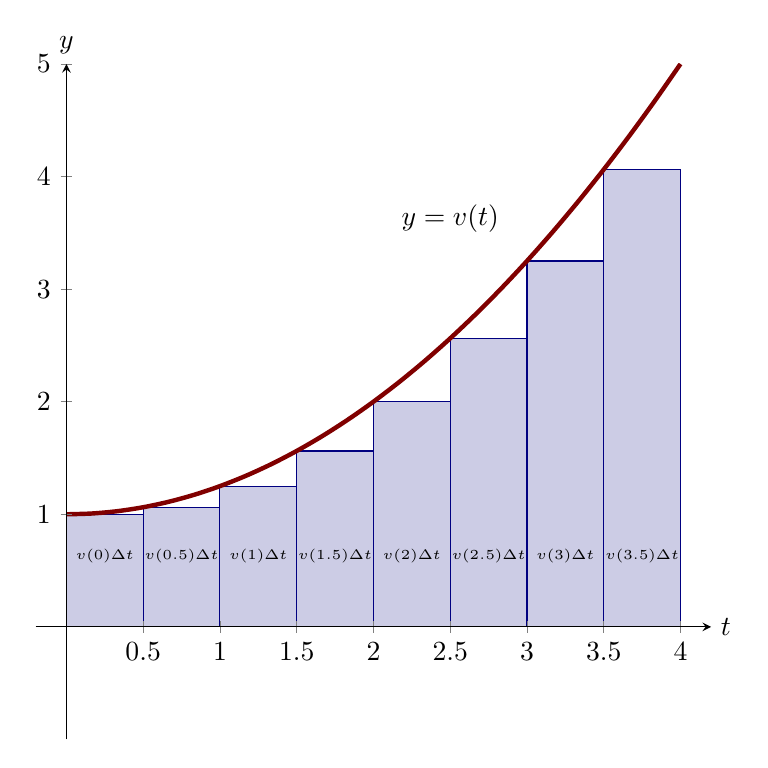
\begin{tikzpicture}[
      declare function = {f(\x) =(1/4)*(x^2) +1;} ]
	\begin{axis}[
            domain=-.2:4.2, xmin =-.2,xmax=4.2,ymax=5,ymin=-1,
            width=4in,
            height=4in,
            xtick={0.5,1,1.5,2,2.5,3,3.5,4}, 
	   ytick={1,2,3,4,5},
            xticklabels={0.5,1,1.5,2,2.5,3,3.5,4},
            yticklabels={1,2,3,4,5},
            axis lines=center, xlabel=$t$, ylabel=$y$,
            every axis y label/.style={at=(current axis.above origin),anchor=south},
            every axis x label/.style={at=(current axis.right of origin),anchor=west},
            axis on top,
          ]
           \addplot [draw=penColor,fill=fillp,domain=0:0.5, smooth] {1} \closedcycle;
           \addplot [draw=penColor,fill=fillp,domain=0.5:1, smooth] {17/16} \closedcycle;
           \addplot [draw=penColor,fill=fillp,domain=1:1.5, smooth] {1.25} \closedcycle;
            \addplot [draw=penColor,fill=fillp,domain=1.5:2, smooth] {25/16} \closedcycle;
             \addplot [draw=penColor,fill=fillp,domain=2:2.5, smooth] {2} \closedcycle;
           \addplot [draw=penColor,fill=fillp,domain=2.5:3, smooth] {41/16} \closedcycle;
           \addplot [draw=penColor,fill=fillp,domain=3:3.5, smooth] {52/16}  \closedcycle;
            \addplot [draw=penColor,fill=fillp,domain=3.5:4, smooth] {65/16} \closedcycle;
          \addplot [ultra thick,penColor2, smooth, domain=0:4] {f(x)};
%%           \addplot [ultra thick,penColor, smooth, domain=0:0.5] {1};
%%             \addplot [ultra thick,penColor, smooth, domain=0.5:1] {17/16};
%% \addplot [ultra thick,penColor, smooth, domain=1:1.5] {1.25};
%% \addplot [ultra thick,penColor, smooth, domain=1.5:2] {25/16};
%% \addplot [ultra thick,penColor, smooth, domain=2:2.5] {2};
%%             \addplot [ultra thick,penColor, smooth, domain=2.5:3] {41/16};
%% \addplot [ultra thick,penColor, smooth, domain=3:3.5] {52/16};
%% \addplot [ultra thick,penColor, smooth, domain=3.5:4] {65/16};
 \node[] at (axis cs:0.25,0.63) {\tiny$v(0)\Delta t$};
   \node[] at (axis cs:.75,0.63) {\tiny$v(0.5)\Delta t$};
   \node[] at (axis cs:1.25,0.63) {\tiny$v(1)\Delta t$};
    \node[] at (axis cs:1.75,0.63) {\tiny$v(1.5)\Delta t$};
     \node[] at (axis cs:2.25,0.63) {\tiny$v(2)\Delta t$};
     \node[] at (axis cs:2.75,0.63) {\tiny$v(2.5)\Delta t$};
     \node[] at (axis cs:3.25,0.63) {\tiny$v(3)\Delta t$};
    \node[] at (axis cs:3.75,0.63) {\tiny$v(3.5)\Delta t$};
                  \node[] at (axis cs:2.5,3.63) {$y=v(t)$};
        \end{axis}
\end{tikzpicture}
\end{image}
We pause here to illustrate the $k$th rectangle when computing a left
Riemann sum of the function $v$ on the interval $[0,4]$.
\begin{image}
  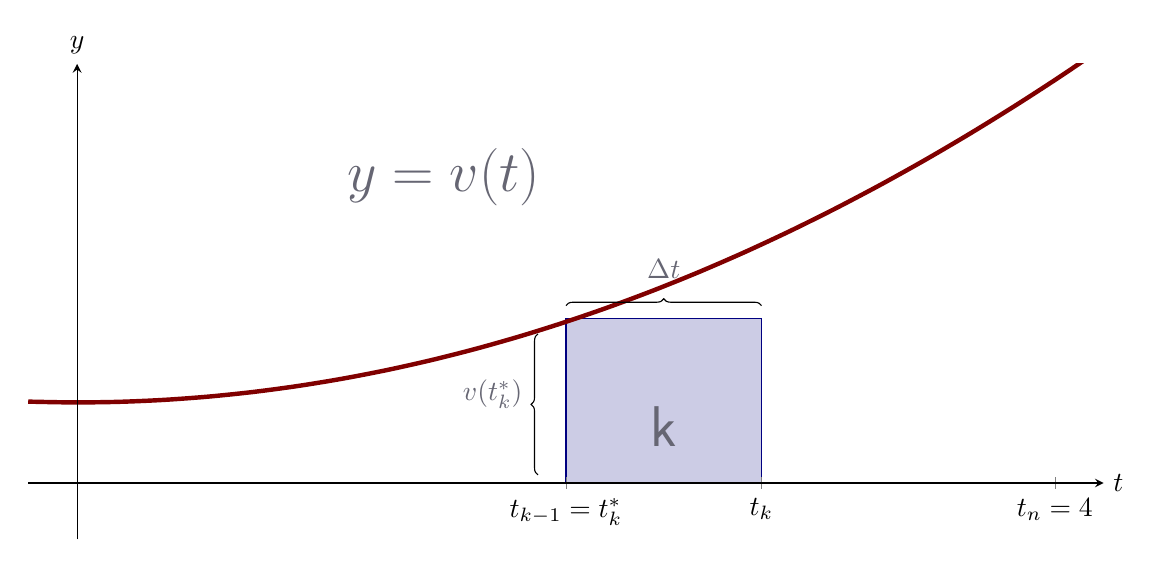
\begin{tikzpicture}[
      declare function = {f(\x) = (1/4)*x^2 + 1;}]
    \begin{axis}[  
        domain=-.2:4.2, xmin =-.2,xmax=4.2,ymax=5.2,ymin=-.7,
        width=6in,
        height=3in,xtick={0,2,2.8,4},
        xticklabels={$t_0=0$,$t_{k-1}=t^*_{k}$,$t_k$,$t_n=4$},
        ytick style={draw=none},
        yticklabels={},
        axis lines=center, xlabel=$t$, ylabel=$y$,
        every axis y label/.style={at=(current axis.above origin),anchor=south},
        every axis x label/.style={at=(current axis.right of origin),anchor=west},
        axis on top,
      ]
      \foreach \rectnumber in {2}
               {
                \addplot [draw=penColor,fill=fillp,domain=2:2.8, smooth] {2.037} \closedcycle;
               };
               \addplot [ultra thick,penColor2, smooth] {f(x)}; 
               %\addplot [ultra thick,penColor2, smooth] plot coordinates {(2,0) (2,2.037)};
               \node[fillp!50!black] at (axis cs:2.4,0.7) {\huge$\mathsf{k}$};
                 \node[fillp!50!black] at (axis cs:1.7,1.1) {${v(t^*_{k})}$};
                  \node[fillp!50!black] at (axis cs:2.4,2.65) {${\Delta t}$};
                   \node[fillp!50!black] at (axis cs:1.5,3.8) {\huge${y=v(t)}$};
                     \addplot[decoration={brace,raise=.2cm},decorate,thin] plot coordinates
                       {(1.95,.1) (1.95,{f(2)-.1})};
               \addplot[decoration={brace,raise=.2cm},decorate,thin] plot coordinates
                       {(2,2.005) (2.8,2.005)};

    \end{axis}
  \end{tikzpicture}
\end{image}

We continue by approximating the displacement of the object assuming
that the velocity is constant during $4/n$-second time intervals, with
velocity equal to the velocity at the beginning of each time interval.


 Under this assumption, during the first $\frac{4}{n}$-second
 interval, the object would move by $v(0)\cdot\frac{4}{n} \unit{ft}$;
 during the second such time interval, the object would move by
 $v\left(\frac{4}{n}\right)\cdot\frac{4}{n} \unit{ft}$, during the
 third time interval, the object would move by
 
 $v\left(2\frac{4}{n}\right)\cdot\frac{4}{n} \unit{ft}$, etc. 
 
 During the entire time interval, the object would move by
\begin{align*}
   \text{displacement} \approx v(0)\cdot\Delta
   t &+v\left(\frac{4}{n}\right)\cdot\Delta
   t+v\left(2\frac{4}{n}\right)\cdot\Delta
   t+\cdots\\
   &+v\left((n-1)\frac{4}{n}\right)\cdot\Delta
   t+v\left(n\frac{4}{n}\right)\cdot\Delta t
\end{align*}
Using sigma notation, notation for the length of each time interval,
$\Delta t=\frac{4-0}{n}=\frac{4}{n}$, and notation for sample pints,
we write

  \[
   \text{displacement}\approx \sum_{k=1}^nv((k-1)\cdot\Delta t)\Delta t
\]
and
\[
   \text{displacement}\approx \sum_{k=1}^nv(t_{k}^*)\Delta t.
  \]
  This is a left Riemann sum for the function $v$ on the interval $[0,4]$.
  
  
What happens when we let $n\to\infty$?

Approximations get better and better, because we approximate the
velocity with a constant over smaller and smaller time intervals.
Therefore, it seems reasonable to write

  \[
   \text{displacement}=\lim_{n\to\infty}\sum_{k=1}^nv(t_k^*)\Delta t
\]

By  the definition of the definite integral, we can write


  \[
   \text{displacement}=\int_{0}^{4}v(t)\d t.
\]

This gives us another interpretation of the definite integral. Namely,



``definite integral of the velocity over $[a,b]$= the displacement over $[a,b]$.''



  On the other hand, the displacement of an object during the time interval $[0,4]$ is given by
  \[
   \text{displacement}=\text{change of position}
\]
  
  The change of position can be written in terms of $s$, the position function of the object
  \[
   \text{displacement}=s(4)-s(0).
\]
But, we know that $s$ is an antiderivative of $v$. Therefore,
 \[
  s(t)=\int v(t)\d t=\int\left(\frac{t^2}{4}+1\right)\d t=\frac{t^3}{\answer[given]{12}}+\answer[given]{t}+C
\]
If $t=0$, we get
 \[
  s(0)=C
\]
So, the position function is given by
\[
  s(t)=\frac{t^3}{\answer[given]{12}}+\answer[given]{t}+s(0).
\]
Now we can compute the displacement
 \[
   \text{displacement}=s(4)-s(0)=\frac{\answer[given]{28}}{3}.
\]
  \end{explanation}
  
Much more important than this computation is the fact that we were able to express the displacement as a definite integral and  compute the definite integral  of $v$ using the antiderivative of $v$.

 \[
   \int_{0}^{4}v(t)\d t=s(4)-s(0)
\]

Is this always so?

Is it true that for any continuous function $f$ and its antiderivative $F$, we can compute the definite integral of $f$ on the interval $[a,b]$ by this simple formula
\[
   \int_{a}^{b}f(t)\d t=F(b)-F(a)?
\]

\end{example}
\end{document}
%
%\begin{example}
%Use your approximation above with a step-size of $dt=2$ to
%estimate $s(10)$.
%\begin{explanation}
%If we label our graph above, we will have a much easier time solving this problem:
%\begin{image}
%  \begin{tikzpicture}[
%      declare function = {f(\x) = 6+\x/2 - pow(\x,2)/4;} ]
%	\begin{axis}[
%        domain=0:10, xmin =0,xmax=10.2,ymax=45,ymin=-1,
%        width=6in,
%        height=3in,
%        xtick={0,2,4,6,8,10}, 
%        %xticklabels={$1$,$1.5$,$2$, $2.5$, $3$},
%        %% ytick style={draw=none},
%        %% yticklabels={},
%        axis lines=center, xlabel=$t$, ylabel=$y$,
%        every axis y label/.style={at=(current axis.above origin),anchor=south},
%        every axis x label/.style={at=(current axis.right of origin),anchor=west},            
%      ]
%      \addplot [draw=penColor,ultra thick] plot coordinates {(0,0) (2,{f(0)*2})};
%      \addplot [draw=penColor2,ultra thick] plot coordinates {(2,{2*f(0)}) (4, {2*f(0)+f(2)*2})};
%      \addplot [draw=penColor3,ultra thick] plot coordinates {(4, {f(0)*2+f(2)*2}) (6, {f(0)*2+f(2)*2+f(4)*2})};
%      \addplot [draw=penColor4,ultra thick] plot coordinates {(6, {f(0)*2+f(2)*2+f(4)*2}) (8, {f(0)*2+f(2)*2+f(4)*2 + f(6)*2})};
%      \addplot [draw=penColor5,ultra thick] plot coordinates {(8, {f(0)*2+f(2)*2+f(4)*2 + f(6)*2}) (10,{f(0)*2+f(2)*2+f(4)*2 + f(6)*2 +f(8)*2} )};
%
%      \addplot [draw=black,dashed,->,>=stealth'] plot coordinates {(.1,0) (1.9, 0)};
%      \addplot [draw=black,dashed,->,>=stealth'] plot coordinates {(2.1,12) (3.9, 12)};
%      \addplot [draw=black,dashed,->,>=stealth'] plot coordinates {(4.1,24) (5.9, 24)};
%      \addplot [draw=black,dashed,->,>=stealth'] plot coordinates {(6.1,32) (7.9, 32)};
%      \addplot [draw=black,dashed,->,>=stealth'] plot coordinates {(8.1,32) (9.9, 32)};
%      
%      \addplot [draw=black,dashed,->,>=stealth'] plot coordinates {(2,1) (2, 11)};
%      \addplot [draw=black,dashed,->,>=stealth'] plot coordinates {(4,13) (4, 23)};
%      \addplot [draw=black,dashed,->,>=stealth'] plot coordinates {(6,25) (6, 31)};
%      \addplot [draw=black,dashed,->, >=stealth'] plot coordinates {(10,31) (10, 21)};
%      
%      \node[anchor=west] at (axis cs:2,6) {\small${\color{penColor}v(0)\cdot 2}$};
%      \node[anchor=west] at (axis cs:4,18) {\small${\color{penColor2}v(2)\cdot 2}$};
%      \node[anchor=west] at (axis cs:6,27) {\small${\color{penColor3}v(4) \cdot 2}$};
%      \node[anchor=east] at (axis cs:8,30) {\small${\color{penColor4}v(6)\cdot 2}$};
%      \node[anchor=east] at (axis cs:10,28) {\small${\color{penColor5}v(8)\cdot 2}$};        
%      
%      \node at (axis cs:5,40) {\Large${\color{penColor}v(0)\cdot 2} + {\color{penColor2}v(2)\cdot 2} + {\color{penColor3}v(4) \cdot 2} + {\color{penColor4}v(6)\cdot 2} + {\color{penColor5}v(8)\cdot 2}$};
%    \end{axis}
%\end{tikzpicture}
%\end{image}
%So
%\begin{align*}
%  s(10) &\approx v(0)\cdot 2 + v(2)\cdot 2 + v(4) \cdot 2 + v(6)\cdot 2 + v(8)\cdot 2\\
%  &= 6\cdot 2 + 6\cdot 2 + 4 \cdot 2 + 0 \cdot 2 +(-6)\cdot 2\\
%  &=\answer[given]{20}.
%\end{align*}
%\end{explanation}
%\end{example}
%
%Hmmm. Let's look at our answer from the previous question again:
%\[
%v(0)\cdot 2 + v(2)\cdot 2 + v(4) \cdot 2 + v(6)\cdot 2 + v(8)\cdot 2
%\]
%\begin{quote}
%  \textbf{This is a Riemann sum!}
%\end{quote}
%When we exclaim (with great excitement!) that ``this is a Riemann
%sum,'' we are really saying that we are in a situation where we may view
%\[
%\text{rate}\times\text{time}
%\]
%as 
%\[
%\text{height}\times\text{width}
%\]
%Check it out: here $n=5$, $\Delta t = 2$, and we are looking at
%left-endpoints! Here is a suggestive graph of $y=v(t)$:    
%\begin{image}
%\begin{tikzpicture}[
%  declare function = {f(\x) = 6+\x/2 - pow(\x,2)/4;}]
%\begin{axis}[  
%    domain=0:10, xmin =-1,xmax=10.2,ymax=10,ymin=-10,
%    width=6in,
%    height=3in,xtick={0,2,4,...,8},
%    xticklabels={$t_1^*=0$,$t_2^*=2$,$t_3^*=4$,$t_4^*=6$,$t_5^*=8$},
%    %% ytick style={draw=none},
%    %% yticklabels={},
%    axis lines=center, xlabel=$t$, ylabel=$y$,
%    every axis y label/.style={at=(current axis.above origin),anchor=south},
%    every axis x label/.style={at=(current axis.right of origin),anchor=west},
%    axis on top,
%  ]
%  \addplot [draw=penColor,fill=fill1] plot coordinates
%           {({1-1) * 2},{f((1-1) * 2)})
%             ({(1) * 2},{f((1-1) * 2) })} \closedcycle;
%
%           \addplot [draw=penColor,fill=fill2] plot coordinates
%           {({2-1) * 2},{f((2-1) * 2)})
%             ({(2) * 2},{f((2-1) * 2) })} \closedcycle;
%
%           \addplot [draw=penColor,fill=fill3] plot coordinates
%           {({3-1) * 2},{f((3-1) * 2)})
%             ({(3) * 2},{f((3-1) * 2) })} \closedcycle;
%
%           \addplot [draw=penColor,fill=fill4] plot coordinates
%           {({4-1) * 2},{f((4-1) * 2)})
%             ({(4) * 2},{f((4-1) * 2) })} \closedcycle;
%
%           \addplot [draw=penColor,fill=fill5] plot coordinates
%           {({5-1) * 2},{f((5-1) * 2)})
%             ({(5) * 2},{f((5-1) * 2) })} \closedcycle;
%           
%           \addplot [ultra thick,penColor, smooth] {f(x)};
%          \node at (axis cs:1,7) {\large$v(0)\cdot 2$};
%          \node at (axis cs:3,7) {\large$v(2)\cdot 2$};
%          \node at (axis cs:5,5) {\large$v(4)\cdot 2$};
%          \node at (axis cs:7,1) {\large$v(6)\cdot 2$};
%          \node at (axis cs:9,1) {\large$v(8)\cdot 2$}; 
%\end{axis}
%\end{tikzpicture}
%\end{image}
%
%Here is the upshot: When we are computing values of antiderivatives,
%we are simultaneously computing areas between curves and the horizontal axis!
%
%\section{On the notation for antiderivatives}
%Let's look at our approximation of $s(t)$ we found above, we'll
%include the actual plot of $s(t)$ as well, shown as a dashed curve:
%\begin{image}
%\begin{tikzpicture}[
%  declare function = {f(\x) = 6+\x/2 - pow(\x,2)/4;} ]
%\begin{axis}[
%    domain=0:10, xmin =0,xmax=10.2,ymax=45,ymin=-1,
%    width=6in,
%    height=3in,
%    xtick={0,2,4,6,8,10}, 
%    %xticklabels={$1$,$1.5$,$2$, $2.5$, $3$},
%    %% ytick style={draw=none},
%    %% yticklabels={},
%    axis lines=center, xlabel=$t$, ylabel=$y$,
%    every axis y label/.style={at=(current axis.above origin),anchor=south},
%    every axis x label/.style={at=(current axis.right of origin),anchor=west},
%  ]
%  \addplot [draw=penColor,ultra thick] plot coordinates {(0,0) (2,{f(0)*2})};
%  \addplot [draw=penColor2,ultra thick] plot coordinates {(2,{2*f(0)}) (4, {2*f(0)+f(2)*2})};
%  \addplot [draw=penColor3,ultra thick] plot coordinates {(4, {f(0)*2+f(2)*2}) (6, {f(0)*2+f(2)*2+f(4)*2})};
%  \addplot [draw=penColor4,ultra thick] plot coordinates {(6, {f(0)*2+f(2)*2+f(4)*2}) (8, {f(0)*2+f(2)*2+f(4)*2 + f(6)*2})};
%  \addplot [draw=penColor5,ultra thick] plot coordinates {(8, {f(0)*2+f(2)*2+f(4)*2 + f(6)*2}) (10,{f(0)*2+f(2)*2+f(4)*2 + f(6)*2 +f(8)*2} )};
%  \addplot [draw=black,ultra thick,dashed] {6*x + x^2/4-x^3/12};
%\end{axis}
%\end{tikzpicture}
%\end{image}    
%At each step we are computing
%\[
%\d s = v(t)\d t
%\]
%and adding it to the previous result:
%\begin{image}
%\begin{tikzpicture}[
%  declare function = {f(\x) = 6+\x/2 - pow(\x,2)/4;} ]
%\begin{axis}[
%    domain=0:10, xmin =0,xmax=10.2,ymax=45,ymin=-1,
%    width=6in,
%    height=3in,
%    xtick={0,2,4,6,8,10}, 
%    %xticklabels={$1$,$1.5$,$2$, $2.5$, $3$},
%    %% ytick style={draw=none},
%    %% yticklabels={},
%    axis lines=center, xlabel=$t$, ylabel=$y$,
%    every axis y label/.style={at=(current axis.above origin),anchor=south},
%    every axis x label/.style={at=(current axis.right of origin),anchor=west},
%  ]
%  \addplot [draw=penColor,ultra thick] plot coordinates {(0,0) (2, 12) (4, 24) (6, 32) (8, 32) (10, 20)};
%
%  \addplot [draw=black,dashed,->,>=stealth'] plot coordinates {(.1,0) (1.9, 0)};
%  \addplot [draw=black,dashed,->,>=stealth'] plot coordinates {(2.1,12) (3.9, 12)};
%  \addplot [draw=black,dashed,->,>=stealth'] plot coordinates {(4.1,24) (5.9, 24)};
%  \addplot [draw=black,dashed,->,>=stealth'] plot coordinates {(6.1,32) (7.9, 32)};
%  \addplot [draw=black,dashed,->,>=stealth'] plot coordinates {(8.1,32) (9.9, 32)};
%
%  \addplot [draw=black,dashed,->,>=stealth'] plot coordinates {(2,1) (2, 11)};
%  \addplot [draw=black,dashed,->,>=stealth'] plot coordinates {(4,13) (4, 23)};
%  \addplot [draw=black,dashed,->,>=stealth'] plot coordinates {(6,25) (6, 31)};
%  \addplot [draw=black,dashed,->, >=stealth'] plot coordinates {(10,31) (10, 21)};
%
%  \node[anchor=west] at (axis cs:2,6) {$\d s$};
%  \node[anchor=west] at (axis cs:4,18) {$\d s$};
%  \node[anchor=west] at (axis cs:6,27) {$\d s$};
%  \node[anchor=east] at (axis cs:8,30) {$\d s$};
%  \node[anchor=east] at (axis cs:10,26) {$\d s$};
%\end{axis}
%\end{tikzpicture}
%\end{image}    
%
%
%
%
%
%If we wanted to, we could take a smaller step-size (our value for
%$dt$) and gain better, and better, approximations of $s(t)$:
%\begin{image}
%\begin{tikzpicture}[
%  declare function = {f(\x) = 6+\x/2 - pow(\x,2)/4;} ]
%\begin{axis}[
%    domain=0:10, xmin =0,xmax=10.2,ymax=45,ymin=-1,
%    width=6in,
%    height=3in,
%    xtick={0,2,4,6,8,10}, 
%    %xticklabels={$1$,$1.5$,$2$, $2.5$, $3$},
%    %% ytick style={draw=none},
%    %% yticklabels={},
%    axis lines=center, xlabel=$t$, ylabel=$y$,
%    every axis y label/.style={at=(current axis.above origin),anchor=south},
%    every axis x label/.style={at=(current axis.right of origin),anchor=west},
%  ]
%  \addplot [draw=black!20!white,ultra thick] plot coordinates {(0,0) (2, 12) (4, 24) (6, 32) (8, 32) (10, 20)};
%  
%  \addplot [draw=black!30!white,ultra thick] plot coordinates {(0,0) (1., 6.) (2., 12.25) (3., 18.25) (4., 23.5) (5., 27.5) (6., 
%    29.75) (7., 29.75) (8., 27.) (9., 21.) (10., 11.25)
%  };
%
%  \addplot [draw=black!40!white,ultra thick] plot coordinates {(0,0) (0.5, 3.) (1., 6.09375) (1.5, 9.21875) (2., 12.3125) (2.5, 
%    15.3125) (3., 18.1563) (3.5, 20.7813) (4., 23.125) (4.5, 25.125) 
%    (5., 26.7188) (5.5, 27.8438) (6., 28.4375) (6.5, 28.4375) (7., 
%    27.7813) (7.5, 26.4063) (8., 24.25) (8.5, 21.25) (9., 17.3438) 
%(9.5, 12.4688) (10., 6.5625)};
%  
%  
%  \addplot [draw=black!50!white,ultra thick] plot coordinates {(0.2, 1.2) (0.4, 2.418) (0.6, 3.65) (0.8, 4.892) (1., 6.14) 
%    (1.2, 7.39) (1.4, 8.638) (1.6, 9.88) (1.8, 11.112) (2., 12.33) 
%    (2.2, 13.53) (2.4, 14.708) (2.6, 15.86) (2.8, 16.982) (3., 
%    18.07) (3.2, 19.12) (3.4, 20.128) (3.6, 21.09) (3.8, 22.002) 
%    (4., 22.86) (4.2, 23.66) (4.4, 24.398) (4.6, 25.07) (4.8, 
%    25.672) (5., 26.2) (5.2, 26.65) (5.4, 27.018) (5.6, 27.3) (5.8, 
%    27.492) (6., 27.59) (6.2, 27.59) (6.4, 27.488) (6.6, 27.28) 
%    (6.8, 26.962) (7., 26.53) (7.2, 25.98) (7.4, 25.308) (7.6, 
%24.51) (7.8, 23.582) (8., 22.52) (8.2, 21.32) (8.4, 19.978) 
%(8.6, 18.49) (8.8, 16.852) (9., 15.06) (9.2, 13.11) (9.4, 
%10.998) (9.6, 8.72) (9.8, 6.272) (10., 3.65)};
%  
%  \addplot [draw=black,ultra thick,dashed] {6*x + x^2/4-x^3/12};
%\end{axis}
%\end{tikzpicture}
%\end{image}
%At this point, we can explain the notation for antiderivatives. If we
%``sum'' all of the ``$\d s$,'' we find the value of position. Hence
%\begin{align*}
%\d s &= v(t) \d t\\
%\text{``sum'' } \d s &= \text{``sum'' } v(t) \d t\\
%\int \d s &= \int v(t) \d t\\
%s(t) &= \int v(t) \d t,
%\end{align*}
%thus we see that an antiderivative is, essentially, a sum.
%
%
%\end{document}
